\clearpage
\thispagestyle{empty}
\phantomsection
\addcontentsline{toc}{chapter}{Yazar Hakkında}
{\Large\bfseries\color{bolumrenk} Yazar Hakkında}
\vspace{0.5cm}
\noindent\rule{\textwidth}{2pt}
\vspace{0.8cm}

\noindent
\raisebox{-\height}{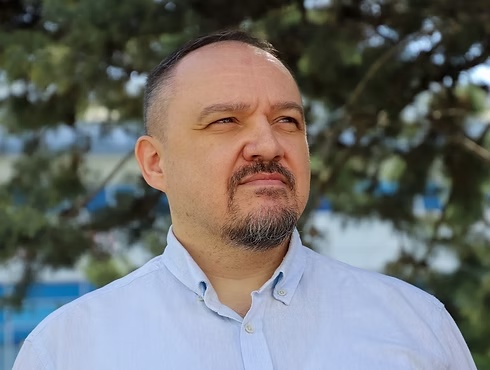
\includegraphics[width=4.5cm]{gorseller/yazar-oguz-ergin.jpg}}%
\hspace{0.7cm}%
\begin{minipage}[t]{10.5cm}%
\textbf{Prof.\ Dr.\ Oğuz Ergin}, bilgisayar mimarisi ve yüksek başarımlı işlemciler üzerine çalışan bir akademisyen, araştırmacı ve girişimcidir. Lisansını ODTÜ'de, yüksek lisans ve doktorasını New York'ta Binghamton Üniversitesi'nde tamamladı. Kariyerinin başında Intel'in Barselona araştırma merkezinde kıdemli araştırmacı olarak çalıştı; Türkiye'ye döndükten sonra TOBB ETÜ'de öğretim üyesi oldu, uzun yıllar bölüm başkanlığı ve üniversite yönetiminde danışmanlık görevleri yürüttü. 2024'ten bu yana Birleşik Arap Emirlikleri'nde Sharjah Üniversitesi Bilgisayar Mühendisliği Bölümü'nde profesör olarak görev yapmaktadır.%
\end{minipage}

\bigskip
\noindent
Araştırmaları; mikroişlemci mimarileri, bellek (özellikle DRAM) güvenliği ve güvenilirliği, enerji verimliliği, donanım hızlandırıcılar ve hata toleransı alanlarına odaklanır. Çalışmaları HPCA, MICRO ve ISCA gibi dünyadaki en saygın konferanslarda yayımlandı; 120'nin üzerinde uluslararası yayını ve çeşitli patentleri bulunmaktadır.

\medskip
\noindent
Akademi-sanayi köprüsünde aktif rol alan Ergin, Kasırga ve Yumruk şirketlerini kurarak savunma ve sivil alanlarda işlemci ve gömülü sistem çözümleri geliştirdi; Aselsan'a ve TUSAŞ'a danışmanlık yaptı ve Bilişim Vadisi'nde teknoloji danışma kurulunda görev aldı. ETH Zürih, Edinburgh ve Notre Dame üniversitelerinde misafir öğretim üyesi olarak bulundu.

\medskip
\noindent
Bugün, yetiştirdiği öğrenciler dünyanın önde gelen araştırma gruplarında ve teknoloji şirketlerinde görev alıyor; danışmanlığını yaptığı öğrenci ekipleri Teknofest yonga tasarımı yarışmalarında birçok derece elde etti. Oğuz Ergin, bilim ve teknoloji temelli yönetim anlayışını; liyakat, şeffaflık ve yüksek katma değerli üretim odaklı bir perspektifle toplumsal faydaya dönüştürmeyi amaçlıyor.
